\subsection{Descripción del problema.}

\vspace*{0.3cm}

Tenemos un enlace por el cual podemos transmitir información, utilizando distintas frecuencias.
Nuestro objetivo es transmitir información durante todo el tiempo que sea posible, pero invirtiendo la menor cantidad de dinero.

Hay que tener en cuenta lo siguiente:

\begin{itemize}
	\item Vamos a transmitir información secuencialmente, es decir que solamente se utilizará UNA frecuencia por intervalo de tiempo.
	\item Cada frecuencia tiene un intervalo $<inicio, fin>$ en el cual puede ser utilizado y un $costo$ por minuto de uso. Los valores $inicio$, $fin$ y $costo$ son números enteros no negativos conocidos de antemano.
	\item El enlace puede eligir transmitir por cualquiera de las frecuencias disponibles, y cambiar de una frecuencia a otra.
	\item Se puede cambiar la frecuencia usada a lo largo del tiempo, pero solo una vez por minuto y al comienzo del mismo.
	\item Se considera tiempo inicial de la transmisión al minuto cero.
	\item la complejidad del algoritmo propuesto debe ser $\mathcal{O}(n*log(n))$.
\end{itemize}

Ejemplo:

Supongamos que tengo una frecuencia 1, con costo por minuto de 10, tiempo de inicio 0 y tiempo final 20, y una frecuencia 2 con costo por minuto 5, tiempo de inicio 5 y tiempo final 10.Entonces nuestra respuesta sería, del minuto 0 al 5 utilizar frecuencia 1, del 5 al 10 utilizar frecuencia 2, y del 10 al 20 utilizar frecuencia 1 nuevamente, ya que de esta manera, se minimizan los costos.


%\begin{figure}[htb]
%  \begin{center}
%      \includegraphics[scale=0.25]{imagenes/ejemplo.jpg}
%  \end{center}
%  \caption{ejemplo}
%\end{figure}

\vspace*{0.6cm}

%\newpage
\subsection{Desarrollo de la idea y pseudocódigo.}

\vspace*{0.3cm}

Nuestro algoritmo debe tomar el intervalo de disponibilidad y el costo de cada frecuencia, para luego indicar qué frecuencia utilizar en cada momento, de manera que la transmisión dure todo el tiempo que sea posible minimizando el costo.

Decidimos representar cada frecuencia con una estructura que contenga sus valores $costo$ (por minuto), $inicio$ y $fin$, además de un valor $nombre$ que identificará a la frecuencia según el orden en el que vino dada.  Para recorrer todas las frecuencias disponibles de una manera cómoda, optamos por tenerlas ordenadas de acuerdo  a su tiempo de $inicio$.  De esta manera, podemos ir recorriéndolas y determinando, mediante comparaciones de sus respectivos costos, cuál ocupará cada intervalo dentro de la transmisión total.

El corazón del algoritmo realiza esta tarea mediante la técnica de {\it Divide \& Conquer}.  La función {\sc frequency_dc} se ocupa de esta etapa (Figura \ref{code:freq_dc}).  Este procedimiento toma un arreglo de frecuencias y lo ``divide'' a la mitad (aproximada en caso de no tener tamaño potencia de 2).  Para cada mitad obtiene, mediante llamadas recursivas, una lista formada por las frecuencias correspondientes, ordenadas y seleccionadas de manera que se transmite la mayor cantidad de tiempo al menor costo.  Teniendo estas dos listas, cada una correspondiente a cada mitad del arreglo de frecuencias, se procede a ``mezclarlas'' de forma tal que seguimos transmitiendo la mayor cantidad de tiempo al menor costo.

Para realizar esta ``mezcla'', que es el trabajo más pesado, utilizamos la función {\sc mezclar_freq} (Figura \ref{code:mezclar}). En ella se crea un iterador al primer elemento de cada sublista recibida para recorrerlas.  Para mayor comodidad en la explicación, llamaremos $trans1$ a la sublista izquierda, $trans2$ a la sublista derecha, y $A$ y $B$ al primer elemento de cada una, respectivamente.

En primera instancia, abordamos 3 casos posibles: 

\begin{enumerate}
\item El tiempo $inicio$ de $A$ y $B$ es el mismo.
\item El tiempo $inicio$ de $A$ es menor al tiempo $inicio$ de $B$.
\item El tiempo $inicio$ de $A$ es mayor al tiempo $inicio$ de $B$ (veremos en breve que este caso puede darse, aunque inicialmente las frecuencias estaban ordenadas de menor a mayor respecto al $inicio$ de cada una).
\end{enumerate}

Estudiemos cada caso por separado:

\vspace*{0.15cm}

{\bf Caso 1: El tiempo $inicio$ de $A$ y $B$ es el mismo.}

\begin{itemize}
\item Si $Costo(A) \leq Costo(B)$:
	\begin{itemize}
	\item Si el tiempo $fin$ de $A$ es menor al tiempo $fin$ de $B$, es conveniente utilizar la frecuencia $A$ por completo y descartar ese intervalo para la frecuencia $B$. Entonces, se elije la frecuencia $A$, se reemplaza el tiempo $inicio$ de $B$ por el tiempo $fin$ de $A$, se mueve el iterador de $trans1$ al siguiente elemento y se prosigue. (Figura \ref{fig:caso1}, 1))
	\item Si el tiempo $fin$ de $A$ es igual al tiempo $fin$ de $B$, es conveniente utilizar la frecuencia $A$, descartando totalmente la frecuencia $B$.  Entonces, se elije la frecuencia $A$, se avanzan ambos iteradores y se prosigue. (Figura \ref{fig:caso1}, 2))
	\item Si el tiempo $fin$ de $A$ es mayor al tiempo $fin$ de $B$, no vale la pena seguir considerando $B$. Entonces, se mueve el iterador de $trans2$ al siguiente elemento y se prosigue. (Figura \ref{fig:caso1}, 3))
	\end{itemize}
\item Si $Costo(A) > Costo(B)$:
	\begin{itemize}
	\item Si el tiempo $fin$ de $A$ es menor al tiempo $fin$ de $B$, no vale la pena seguir considerando $A$. Entonces, se mueve el iterador de $tran1$ al siguiente elemento y se prosigue (Figura \ref{fig:caso1}, 4)). Notar que en este caso, suponiendo que ambas listas tienen más de un elemento, en la siguiente iteración se comparará el siguiente elemento de $trans1$ (llamémoslo $AA$) contra $B$.  Como $A$ y $B$ tienen el mismo inicio, si consideramos que los intervalos no son vacíos, $fin$ de $A$ debe ser mayor a $inicio$ de $A$, y como $inicio$ de $AA$ debe ser mayor o igual a $fin$ de $A$, deducimos que $inicio$ de $AA$ es mayor a $inicio$ de $B$.  Este es uno de los casos en los que será necesario considerar la opción 3 de los casos establecidos anteriormente.
	\item Si el tiempo $fin$ de $A$ es igual al tiempo $fin$ de $B$, es conveniente utilizar la frecuencia $B$, descartando totalmente la frecuencia $A$.  Entonces, se elije la frecuencia $B$, se avanzan ambos iteradores y se prosigue. (Figura \ref{fig:caso1}, 5))
	\item Si el tiempo $fin$ de $A$ es mayor al tiempo $fin$ de $B$, es conveniente utilizar la frecuencia $B$ por completo y descartar ese intervalo para la frecuencia $A$. Entonces, se elije la frecuencia $B$, se reemplaza el tiempo $inicio$ de $A$ por el tiempo $fin$ de $B$, se mueve el iterador de $trans2$ al siguiente elemento y se prosigue. (Figura \ref{fig:caso1}, 6))
	\end{itemize}
\end{itemize}

\begin{figure}[htb]
  \begin{center}
      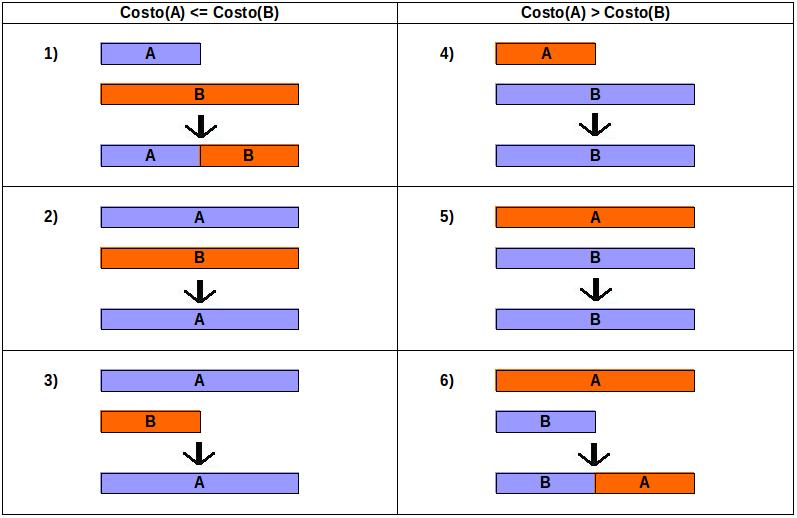
\includegraphics[scale=0.5]{imagenes/caso1.jpeg}
  \end{center}
  \caption{Ilustración de las posibles elecciones en el caso 1}\label{fig:caso1}
\end{figure}
%\FloatBarrier

{\bf Caso 2: El tiempo $inicio$ de $A$ es menor al tiempo $inicio$ de $B$.}

Si el tiempo $fin$ de $A$ es menor al tiempo $inicio$ de $B$, significa que ambas frecuencias no entran en conflicto, así que se elije la frecuencia $A$, se avanza el iterador de $trans1$ y se prosigue.

Si el tiempo $fin$ de $A$ es mayor al tiempo $inicio$ de $B$, tenemos las siguientes situaciones:

\begin{itemize}
\item Si $Costo(A) \leq Costo(B)$, se procede de la misma forma que en el caso 1. (Figura \ref{fig:caso2},1-3)
\item Si $Costo(A) > Costo(B)$:
	\begin{itemize}
	\item Si el tiempo $fin$ de $A$ es menor al tiempo $fin$ de $B$, es conveniente usar la frecuencia $B$ y descartar ese intervalo de la frecuencia $A$.  Entonces, se elije la frecuencia $A$ modificando su $fin$ por el $inicio$ de $B$, se avanza el iterador de $trans1$ y se prosigue (Figura \ref{fig:caso3},4).  Nuevamente, nos encontramos ante un caso en el cual el iterador de $trans1$ queda apuntando a un elemento con $inicio$ mayor al $inicio$ de $B$, y se vuelve necesario contemplar el caso 3.
	\item Si el tiempo $fin$ de $A$ es igual al tiempo $fin$ de $B$, es conveniente usar la frecuencia $B$ y descartar ese intervalo de la frecuencia $A$.  Entonces, se toma la frecuencia $A$ modificando su $fin$ por el $inicio$ de $B$, se elije luego $B$, se avanzan ambos iteradores y se prosigue.
	\item Si el tiempo $fin$ de $A$ es mayor al tiempo $fin$ de $B$, es conveniente utilizar la frecuencia $B$ por completo y descartar ese intervalo para la frecuencia $A$. Entonces, se toma la frecuencia $A$ hasta el comienzo de la frecuencia $B$, luego se toma la frecuencia $B$ completamente, se modifica el $inicio$ de $A$ por el $fin$ de $B$, se avanza el iterador de $trans2$ y se prosigue. (Figura \ref{fig:caso2}, 1))
	\end{itemize}
\end{itemize}

\begin{figure}[htb]
  \begin{center}
      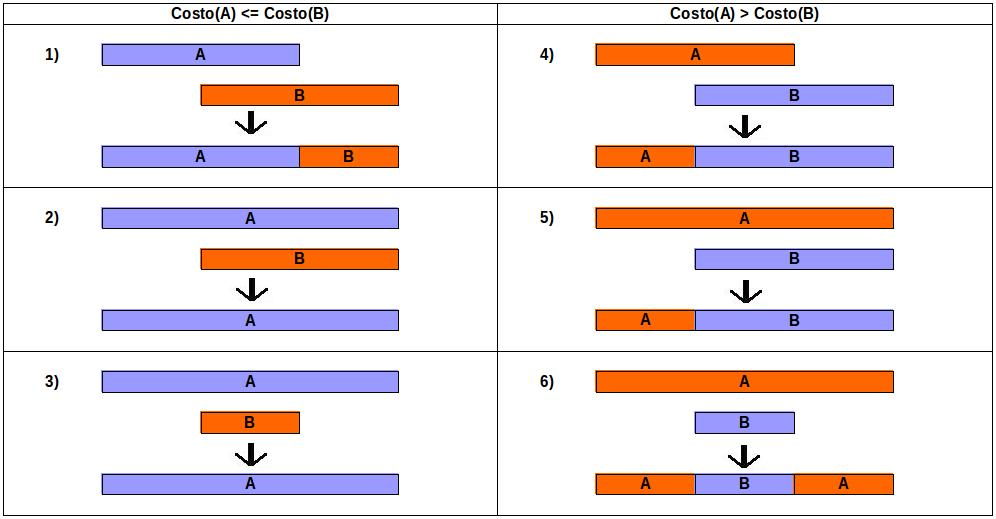
\includegraphics[scale=0.5]{imagenes/caso2.jpeg}
  \end{center}
  \caption{Ilustración de las posibles elecciones en el caso 2}\label{fig:caso2}
\end{figure}
%\FloatBarrier

{\bf Caso 3: El tiempo $inicio$ de $A$ es mayor al tiempo $inicio$ de $B$.}

\begin{itemize}
\item Si $Costo(A) < Costo(B)$:
	\begin{itemize}
	\item Si el tiempo $fin$ de $A$ es menor al tiempo $fin$ de $B$, es conveniente utilizar la frecuencia $A$ por completo y descartar ese intervalo para la frecuencia $B$. Entonces, se toma la frecuencia $B$ hasta el comienzo de la frecuencia $A$, luego se toma la frecuencia $A$ completamente, se modifica el $inicio$ de $B$ por el $fin$ de $A$, se avanza el iterador de $trans1$ y se prosigue. (Figura \ref{fig:caso3}, 1))
	\item Si el tiempo $fin$ de $A$ es igual al tiempo $fin$ de $B$, es conveniente utilizar la frecuencia $B$ hasta el $inicio$ de $A$ para luego utilizar por completo la frecuencia $A$. Entonces, se procede de la manera indicada, se avanzan ambos iteradores y se prosigue. (Figura \ref{fig:caso3}, 2))
	\item Si el tiempo $fin$ de $A$ es mayor al tiempo $fin$ de $B$, conviene utilizar la frecuencia $B$ hasta el $inicio$ de $A$ para luego utilizar por completo la frecuencia $A$.  Entonces, se toma la frecuencia $B$ hasta el $inicio$ de $A$, se avanza el iterador de $trans2$ y se prosigue. (Figura \ref{fig:caso3}, 3))
	\end{itemize}
\item Si $Costo(A) \geq Costo(B)$:
	\begin{itemize}
	\item Si el tiempo $fin$ de $A$ es menor al tiempo $fin$ de $B$, no vale la pena seguir considerando $A$. Entonces, se mueve el iterador de $tran1$ al siguiente elemento y se prosigue (Figura \ref{fig:caso3}, 4)). 		\item Si el tiempo $fin$ de $A$ es igual al tiempo $fin$ de $B$, es conveniente utilizar la frecuencia $B$, descartando totalmente la frecuencia $A$.  Entonces, se elije la frecuencia $B$, se avanzan ambos iteradores y se prosigue. (Figura \ref{fig:caso3}, 5))
	\item Si el tiempo $fin$ de $A$ es mayor al tiempo $fin$ de $B$, es conveniente utilizar la frecuencia $B$ por completo y descartar ese intervalo para la frecuencia $A$. Entonces, se elije la frecuencia $B$, se reemplaza el tiempo $inicio$ de $A$ por el tiempo $fin$ de $B$, se mueve el iterador de $trans2$ al siguiente elemento y se prosigue. (Figura \ref{fig:caso3}, 6))
	\end{itemize}
\end{itemize}

\begin{figure}[htb]
  \begin{center}
      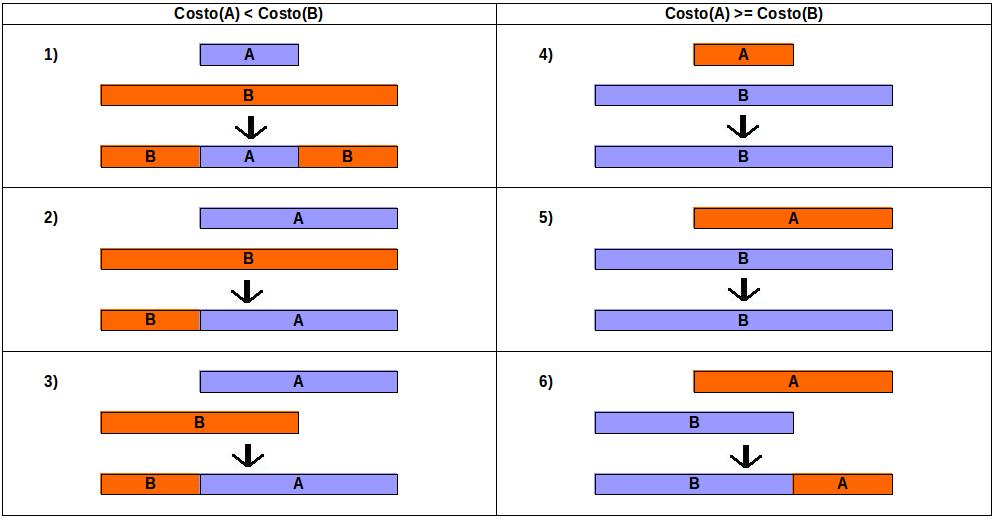
\includegraphics[scale=0.5]{imagenes/caso3.jpeg}
  \end{center}
  \caption{Ilustración de las posibles elecciones en el caso 3}\label{fig:caso3}
\end{figure}
%\FloatBarrier

\begin{figure}[!ht]
\begin{codebox}
\Procname{$\proc{frecuency_dc}(Arreglo$_$frecuencias$ $freq, int$ $low, int$ $high)$}
\li trans1,trans2,trans_final $\leftarrow$ listas vacías de frecuencias
\li \If ($low < high$)
\li		\Then 
			mitad $\leftarrow$ $\dfrac{low + high}{2}$
\li			trans1 $\leftarrow$ $frequency$_$dc(freq,low,mitad)$
\li			trans2 $\leftarrow$ $frequency$_$dc(freq,mitad+1,high)$
\li			trans_final $\leftarrow$ {\sc mezclar_freq}(trans1,trans2)
\li 		\Else
			trans_final $\leftarrow$ agregar la única frecuencia dada.
		\End
\li \Return trans_final 
 \end{codebox}
\caption{Pseudocódigo de frequency_dc}\label{code:freq_dc}
\end{figure}
%\FloatBarrier

\begin{figure}[!ht]
\begin{codebox}
\Procname{$\proc{mezclar_freq}(Lista$_$frecuencia$ $trans1, Lista$_$frecuencia$ $trans2)$}
\li res $\leftarrow$ lista vacía de frecuencias
\li it1 $\leftarrow$ iterador a trans1
\li it2 $\leftarrow$ iterador a trans2
\li \While it1 e it2 sean válidos
\li		\Do 
 		\If ((it1$\rightarrow$inicio) == (it2$\rightarrow$inicio))
\li 			\Then
				\If ((it1$\rightarrow$costo) $\leq$ (it2$\rightarrow$costo))
\li					\Then {\sc aux_mezcla_a}(it1,it2,res)
\li				\Else
					{\sc aux_mezcla_a}(it2,it1,res)
				\End
\li 			\Else
				\If ((it1$\rightarrow$inicio) $<$ (it2$\rightarrow$inicio))
\li				\Then
					\If ((it1$\rightarrow$fin) $\leq$ (it2$\rightarrow$inicio))
\li					\Then
						res $\leftarrow$ agregar al final el dato de it1
\li						avanzar it1
\li					\Else
\li 						\If ((it1$\rightarrow$costo) $\leq$ (it2$\rightarrow$costo))
\li							\Then {\sc aux_mezcla_a}(it1,it2,res)
\li							\Else
								{\sc aux_mezcla_b}(it1,it2,res)
							\End
					\End
\li 				\Else 
\li					\If ((it1$\rightarrow$costo) $<$ (it2$\rightarrow$costo))
\li 						\Then {\sc aux_mezcla_b}(it2,it1,res)
\li 						\Else
 							{\sc aux_mezcla_a}(it2,it1,res)
 						\End
 				\End
 			\End
 		\End
\li \If alguna de las listas no fue recorrida totalmente
\li 		\Then res $\leftarrow$ agregar remanente de esa lista
		\End
\li \Return res
\end{codebox}
\caption{Pseudocódigo de mezclar_freq} \label{code:mezclar}
\end{figure}
%\FloatBarrier

\begin{figure}[!ht]
\begin{codebox}
\Procname{$\proc{aux_mezcla_a}(it$_$Lista$_$frecuencia$ $itA, it$_$Lista$_$frecuencia$ $itB, Lista$_$frecuencia$ $res)$}
\li	\If((itA$\rightarrow$fin) $<$ (itB$\rightarrow$fin))
\li 		\Then
			res $\leftarrow$ agregar atrás el dato de itA
\li 			(itB$\rightarrow$inicio) $\leftarrow$ (itA$\rightarrow$fin)
\li			avanzar itA
\li 		\Else
			\If ((itA$\rightarrow$fin) == (itB$\rightarrow$fin)
\li				res $\leftarrow$ agregar atrás el dato de itA
\li 				avanzar itA
\li 				avanzar itB
\li 		\Else avanzar itB
		\End
\li		\Return
\end{codebox}

\begin{codebox}
\Procname{$\proc{aux_mezcla_b}(it$_$Lista$_$frecuencia$ $itA, it$_$Lista$_$frecuencia$ $itB, Lista$_$frecuencia$ $res)$}
\li res $\leftarrow$ agregar atrás el dato de itA
\li (res.último_elemento)$\rightarrow$fin $\leftarrow$ (itB$\rightarrow$inicio)
\li	\If((itA$\rightarrow$fin) $<$ (itB$\rightarrow$fin))
\li 		\Then avanzar itA
\li 		\Else
			\If ((itA$\rightarrow$fin) == (itB$\rightarrow$fin)
\li				res $\leftarrow$ agregar atrás el dato de itB
\li 				avanzar itA
\li 				avanzar itB
\li 		\Else 
			res $\leftarrow$ agregar atrás el dato de itA
\li 			(itA$\rightarrow$inicio) $\leftarrow$ (itB$\rightarrow$fin)
\li			avanzar itB
		\End
\li		\Return
\end{codebox}
\caption{Pseudocódigo de las funciones auxiliares a mezclar_freq} \label{code:aux}
\end{figure}
%\FloatBarrier

\vspace*{0.6cm}

%\newpage
\subsection{Justificación de la resolución y demostración de correctitud.}

\vspace*{0.3cm}



\vspace*{0.6cm}

%\newpage
\subsection{Análisis de complejidad.}

\vspace*{0.3cm}

En este apartado demostraremos que la complejidad total de nuestro algoritmo es $\mathcal{O}(n*log(n))$.

Empezaremos analizando el pseudocódigo de AltaFrecuencia (Figura \ref{code:altafrec}) asumiendo que la complejidad de frecuency_dc es $\mathcal{O}(n*log(n))$
En las dos primeras lineas se procede a crear una lista vacía $\mathcal{O}(1)$ y una lista que se completará con las frecuencias tomadas de la entrada. Esto último requiere recorrer la entrada $\mathcal{O}(n)$ y copiar los datos $\mathcal{O}(1)$.
En la línea 3 de la figura se pasa a ordenar la lista en base a los tiempos de inicio de cada elemento $\mathcal{O}(n*log(n))$ para luego en la línea 4 ser trasladada a un arreglo previamente creado $\mathcal{O}(n)$. Con dicho arreglo y la función frecuency_dc se arma lo que será la lista solución del problema $\mathcal{O}(n*log(n))$. A continuación, se recorre la lista solución calculando el costo total de la transmisión $\mathcal{O}(n)$ para luego, en la línea 8 mostrar ese valor junto con las frecuencias utilizadas. Esto último se considera $\mathcal{O}(n)$ ya que los costos de mostrar datos son tomados como $\mathcal{O}(1)$ y el costo de recorrer la solución es $\mathcal{O}(n)$.

\begin{figure}[!ht]
\begin{codebox}
\Procname{$\proc{AltaFrecuencia}()$} 
\li Creo una lista de transmisiones resultado  //$\mathcal{O}(1)$ 
\li freq_l $\leftarrow$ Creo una lista para almacenar las n frecuencias levantadas de la entrada
\li ordeno_por_tiempo(freq_l) {\it //ordeno por tiempo de inicio. $\mathcal{O}(n.logn)$}
\li total_freq $\leftarrow$ paso freq_l ordenada a un arreglo $\mathcal{O}(n)$
\li resultado $\leftarrow$ frecuency_dc(total_freq,0,n-1)
\li {\it //armo la transmisión resultado haciendo uso de la técnica de D\&C}
\li costo_total $\leftarrow$ costo_transmision(resultado) //$\mathcal{O}(n)$
\li Muestro por pantalla: costo de la transmisión (costo_total) y el intervalo de tiempo ocupado por cada\\ frecuencia usada {\it //Se hace en $\mathcal{O}(n)$ porque es recorrer la lista mostrando las frecuencias $\mathcal{O}(1)$}
\end{codebox}
\caption{Pseudocódigo de AltaFrecuencia}\label{code:altafrec}
\end{figure}
\FloatBarrier

Luego con la siguiente ecuación:

\begin{equation*}
\begin{array}{l}
T(n) = \mathcal{O}(1) + 2\mathcal{O}(n)*\mathcal{O}(1) + 2\mathcal{O}(n*log(n)) + 3\mathcal{O}(n)\\
T(n) = \mathcal{O}(n*log(n))
\end{array}
\end{equation*}

La complejidad total de este algoritmo es, entonces, $\mathcal{O}(n*log(n))$.

Resta ver que frecuency_dc es en efecto $\mathcal{O}(n*log(n))$.


\vspace*{0.6cm}

%\newpage
\subsection{Experimentación y gráficos.}

\vspace*{0.3cm}

\subsubsection{Test 1}

\vspace*{0.3cm}

\textbf{completar!}


\newpage
\subsubsection{Test 2}

\vspace*{0.3cm}

\textbf{completar!}


\newpage
\subsubsection{Test 3}

\vspace*{0.3cm}

\textbf{completar!}
